%%%%%%%%%%%%%%%%%%%%%%%%%%%%%%%%%%%%%%%%%%%%%%%%%%
% Title page template been downloaded from:
% http://www.LaTeXTemplates.com
%%%%%%%%%%%%%%%%%%%%%%%%%%%%%%%%%%%%%%%%%%%%%%%%%%

\documentclass[a4paper]{article}
\RequirePackage[utf8]{inputenc}
\usepackage[portuguese]{babel}
\usepackage{listings}
\usepackage{color}
\usepackage{graphicx}
\usepackage{hyperref}
\usepackage{helvet}
\usepackage{fullpage}
\renewcommand{\familydefault}{\sfdefault}

\definecolor{dkgreen}{rgb}{0,0.6,0}
\definecolor{gray}{rgb}{0.5,0.5,0.5}
\definecolor{mauve}{rgb}{0.58,0,0.82}

\lstset{frame=tb,
  language=Java,
  aboveskip=3mm,
  belowskip=3mm,
  showstringspaces=false,
  columns=flexible,
  basicstyle={\small\ttfamily},
  numbers=none,
  numberstyle=\tiny\color{gray},
  keywordstyle=\color{blue},
  commentstyle=\color{dkgreen},
  stringstyle=\color{mauve},
  breaklines=true,
  breakatwhitespace=true,
  tabsize=3,
  literate=
  {á}{{\'a}}1 {é}{{\'e}}1 {í}{{\'i}}1 {ó}{{\'o}}1 {ú}{{\'u}}1
  {Á}{{\'A}}1 {É}{{\'E}}1 {Í}{{\'I}}1 {Ó}{{\'O}}1 {Ú}{{\'U}}1
  {à}{{\`a}}1 {è}{{\'e}}1 {ì}{{\`i}}1 {ò}{{\`o}}1 {ù}{{\`u}}1
  {À}{{\`A}}1 {È}{{\'E}}1 {Ì}{{\`I}}1 {Ò}{{\`O}}1 {Ù}{{\`U}}1
  {ä}{{\"a}}1 {ë}{{\"e}}1 {ï}{{\"i}}1 {ö}{{\"o}}1 {ü}{{\"u}}1
  {Ä}{{\"A}}1 {Ë}{{\"E}}1 {Ï}{{\"I}}1 {Ö}{{\"O}}1 {Ü}{{\"U}}1
  {â}{{\^a}}1 {ê}{{\^e}}1 {î}{{\^i}}1 {ô}{{\^o}}1 {û}{{\^u}}1
  {Â}{{\^A}}1 {Ê}{{\^E}}1 {Î}{{\^I}}1 {Ô}{{\^O}}1 {Û}{{\^U}}1
  {œ}{{\oe}}1 {Œ}{{\OE}}1 {æ}{{\ae}}1 {Æ}{{\AE}}1 {ß}{{\ss}}1
  {ç}{{\c c}}1 {Ç}{{\c C}}1 {ø}{{\o}}1 {å}{{\r a}}1 {Å}{{\r A}}1
  {€}{{\EUR}}1 {£}{{\pounds}}1
}

\begin{document}

\begin{titlepage}

\newcommand{\HRule}{\rule{\linewidth}{0.5mm}} % Defines a new command for the horizontal lines, change thickness here

\center % Center everything on the page
 
%----------------------------------------------------------------------------------------
%	HEADING SECTIONS
%----------------------------------------------------------------------------------------

\textbf{\Large INSTITUTO SUPERIOR DE ENGENHARIA DE LISBOA}\\[1cm] % Name of your university/college
\textbf{ Área Departamental de Engenharia de Electrónica e Telecomunicações e de Computadores 
}\\[0.5cm] % Major heading such as course name

\textbf{Licenciatura de Engenharia Informática e Computadores}\\[2.5cm]

%----------------------------------------------------------------------------------------
%	TITLE SECTION
%----------------------------------------------------------------------------------------

\textbf{\large Unidade Curricular de Sistemas Distribuídos }

\textbf{(2º semestre lectivo 2013/2014)}\\[3cm]


\textbf{\huge Protocolo Websocket}\\[5cm]
 
%----------------------------------------------------------------------------------------
%	AUTHOR SECTION
%----------------------------------------------------------------------------------------




{\raggedright{}
	\textbf{Grupo G03D:}
	
	\textbf{32632 Pedro Pedroso} 

	\textbf{33404 Ricardo Mata}

	\textbf{33724 David Raposo}\\[5cm]
}



%----------------------------------------------------------------------------------------
%	DATE SECTION
%----------------------------------------------------------------------------------------
{\large \today}\\[3cm] % Date, change the \today to a set date if you want to be precise

\vfill % Fill the rest of the page with whitespace

\end{titlepage}


%----------------------------------------------------------------------------------------
%	BODY
%----------------------------------------------------------------------------------------
\newpage
\setcounter{page}{1} %começa a contar as páginas apartir do 1

\section{Resumo}

Com este trabalho pretendemos fazer uma síntese do protocolo \emph{WebSocket}. O objectivo deste protocolo é disponibilizar um meio de ter uma ligação que seja full-duplex (comunicação pode ser feita nos dois sentidos) utilizando um só socket assim como simplificar o processo.

É um protocolo baseado em tcp, utilizando HTTP somente durant o \emph{handshake}.

\begin{itemize}
\item Apresentar a sua estrutura
\item Apresentar e discutir vantagens/desvantagens
\end{itemize}

%----------------------------------------------------------------------------------------
\newpage

\section{\emph{WebSocket} }

\section{\emph{Handshake}}
\textsf{A ligação inicial é realizada como uma ligação HTTP. Isto acontece para assegurar compatibilidade com protocolos mais antigos. Depois do contacto, é enviado um \emph{request} para que o protocolo seja alterado para websocket através do seguinte \emph{header}:}\\[0.5cm]

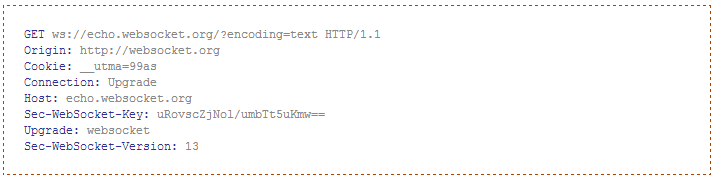
\includegraphics[height=3.5cm]{websocketUpdateRequest}

\textsf{text text text}\\[0.5cm]

\includegraphics[height=3.5cm]{websocketUpdateResponse}


%----------------------------------------------------------------------------------------
\newpage
\section{Conclusões}

\textsf{Concluo o trabalho aqui}

%----------------------------------------------------------------------------------------
\newpage

\section{Bibliografia}

\textsf{Este documento foi escrito com base na informação presente nos seguintes recursos:}
\begin{itemize}
\item \url{http://www.websocket.org/aboutwebsocket.html}
\end{itemize}


\end{document}